%%%%%%%%%%%%%%%%%%%%%%%%%%%%%%%%%%%%%%%%%%%%%%%%%%%%%%%%%%%%%%%%%%%%%%%%%%%%%%%%%%
\begin{frame}[fragile]\frametitle{}
\begin{center}
{\Large Concepts}
\end{center}
\end{frame}


%%%%%%%%%%%%%%%%%%%%%%%%%%%%%%%%%%%%%%%%%%%%%%%%%%%%%%%%%%%
\begin{frame}[fragile]\frametitle{Cost-Efficient GraphRAG Approach}
    \begin{itemize}
        \item Leverages graphs for RAG without high costs.
        \item Minimizes reliance on LLMs or uses smaller on-premise models.
        \item Structured as a layered graph:
        \begin{itemize}
            \item Ontology Layer – Defines domain structure (fixed or nearly fixed).
            \item Document Layer – Contains chunked documents, similar to a vector DB.
            \item Entity Layer (Optional) – Extracted entities enhance search.
        \end{itemize}
    \end{itemize}
\end{frame}

%%%%%%%%%%%%%%%%%%%%%%%%%%%%%%%%%%%%%%%%%%%%%%%%%%%%%%%%%%%
\begin{frame}[fragile]\frametitle{Challenges in Ontology-Based Graphs}
    \begin{itemize}
        \item Not all datasets belong to a well-defined domain.
        \item Subject Matter Experts (SMEs) may not be available.
        \item Eliminating fixed ontology layer could improve flexibility.
    \end{itemize}
\end{frame}

%%%%%%%%%%%%%%%%%%%%%%%%%%%%%%%%%%%%%%%%%%%%%%%%%%%%%%%%%%%
\begin{frame}[fragile]\frametitle{NLP-Powered Graph Approach}
    \begin{itemize}
        \item Drops the ontology layer for cost-efficiency.
        \item Graph consists of:
        \begin{itemize}
            \item Document Layer – Contains document chunks.
            \item Tokens Layer – Extracted tokens improve search.
        \end{itemize}
        \item NLP reduces dependency on LLMs.
    \end{itemize}
\end{frame}

%%%%%%%%%%%%%%%%%%%%%%%%%%%%%%%%%%%%%%%%%%%%%%%%%%%%%%%%%%%
\begin{frame}[fragile]\frametitle{Data Preprocessing Pipeline}
    \begin{itemize}
        \item Chunking – Splitting documents into segments.
        \item Embedding – Using Hugging Face model for embeddings.
        \item Graph Construction – Built using NetworkX or Neo4j.
        \item Token Extraction – Generates token, bigram, and trigram nodes.
    \end{itemize}
\end{frame}

%%%%%%%%%%%%%%%%%%%%%%%%%%%%%%%%%%%%%%%%%%%%%%%%%%%%%%%%%%%
\begin{frame}[fragile]\frametitle{Indexing and Interconnectivity}
    \begin{itemize}
        \item Tokens are shared across documents, interlinking content.
        \item Need to connect entities using context, logic, and semantics.
        \item Avoid reliance on massive models due to cost constraints.
    \end{itemize}
\end{frame}

%%%%%%%%%%%%%%%%%%%%%%%%%%%%%%%%%%%%%%%%%%%%%%%%%%%%%%%%%%%
\begin{frame}[fragile]\frametitle{Triple Extraction for Graph Optimization}
    \begin{itemize}
        \item Triple extraction improves retrieval efficiency.
        \item Uses a smaller transformer model fine-tuned for this task.
        \item Triplets mapped to token nodes enhance query performance.
        \item Queries traverse graph using triplet relationships.
    \end{itemize}
\end{frame}

%%%%%%%%%%%%%%%%%%%%%%%%%%%%%%%%%%%%%%%%%%%%%%%%%%%%%%%%%%%
\begin{frame}[fragile]\frametitle{Optimizing Graph-Based Retrieval}
    \begin{itemize}
        \item Combines standard RAG with triplet-enhanced retrieval.
        \item Retrieves relevant text chunks and connected triplets.
        \item Improves search relevance and reduces retrieval complexity.
    \end{itemize}
\end{frame}

%%%%%%%%%%%%%%%%%%%%%%%%%%%%%%%%%%%%%%%%%%%%%%%%%%%%%%%%%%%%%%%%%%%%%%%%%%%%%%%%%%
\begin{frame}[fragile]\frametitle{}
\begin{center}
{\Large Approaches}
\end{center}
\end{frame}


%%%%%%%%%%%%%%%%%%%%%%%%%%%%%%%%%%%%%%%%%%%%%%%%%%%%%%%%%%%
\begin{frame}[fragile]\frametitle{}

	\begin{center}
	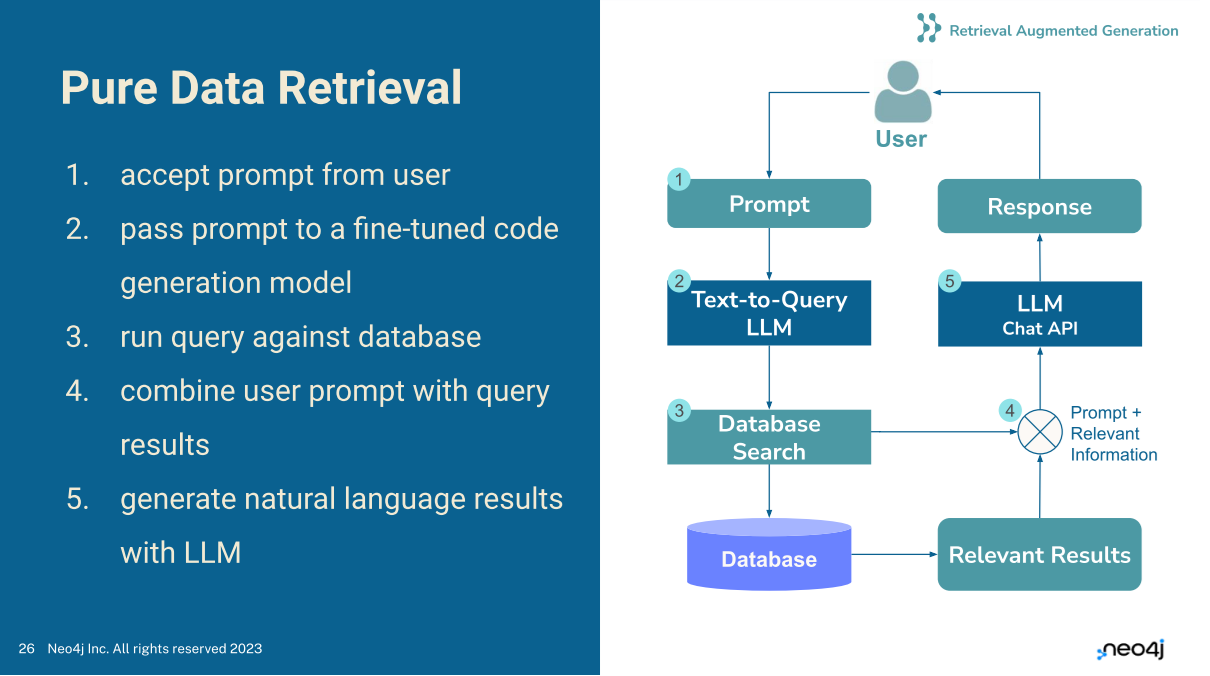
\includegraphics[width=\linewidth,keepaspectratio]{graphrag3}
	\end{center}
	
	
\end{frame}

%%%%%%%%%%%%%%%%%%%%%%%%%%%%%%%%%%%%%%%%%%%%%%%%%%%%%%%%%%%
\begin{frame}[fragile]\frametitle{Challenges}
    \begin{itemize}
        \item Getting it to work at all – generating syntactically correct queries
        \item Getting it to do the right thing – producing meaningful results
        \item Avoiding accidents – mistaken deletion
        \item Preventing malicious intent – SQL injection gone wild
    \end{itemize}
	
	{\tiny (Ref: The GenAI Stack - Andreas Kollegger - Neo4j)}
	
\end{frame}


%%%%%%%%%%%%%%%%%%%%%%%%%%%%%%%%%%%%%%%%%%%%%%%%%%%%%%%%%%%
\begin{frame}[fragile]\frametitle{}

	\begin{center}
	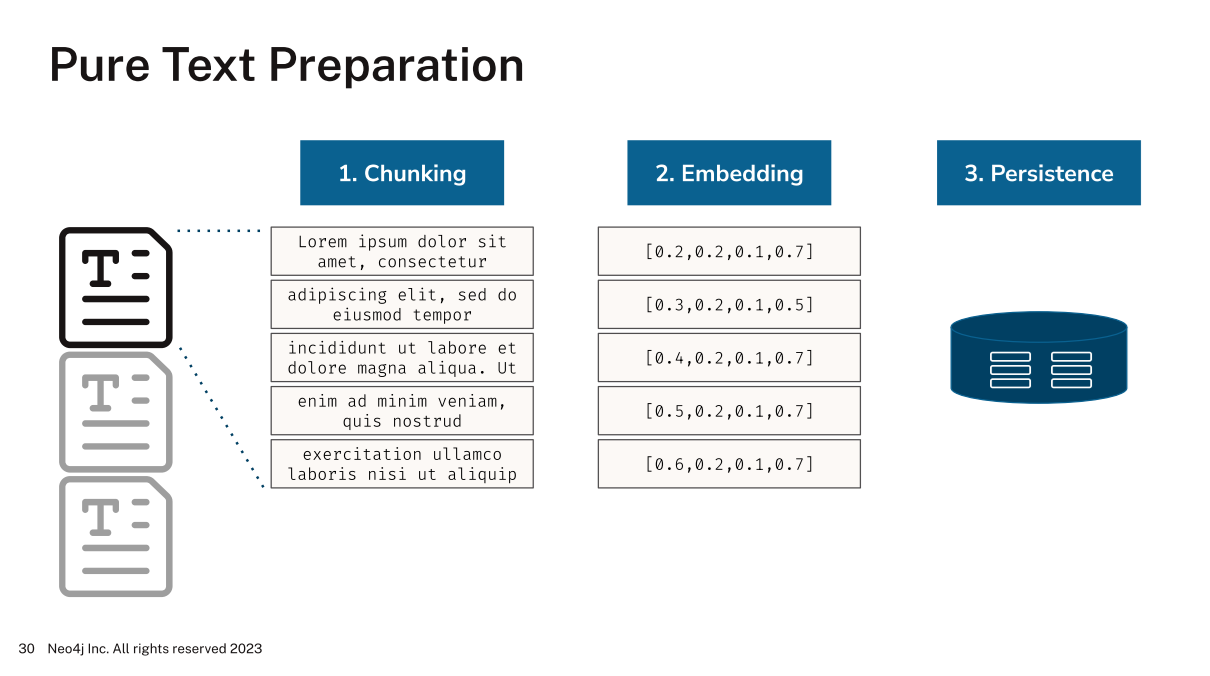
\includegraphics[width=\linewidth,keepaspectratio]{graphrag4}
	\end{center}
	
\end{frame}

%%%%%%%%%%%%%%%%%%%%%%%%%%%%%%%%%%%%%%%%%%%%%%%%%%%%%%%%%%%
\begin{frame}[fragile]\frametitle{Challenges}
    \begin{itemize}
        \item How?
		    \begin{itemize}
				\item pick a chunk method \& size
				\item each chunk is a record
				\item store chunk with metadata
				\item connect each chunk to original document
				\item connect previous/next chunk
		    \end{itemize}
        \item Challenges:
		    \begin{itemize}
				\item what makes a good chunk?
				\item potential chunk duplication
				\item how to re-assemble chunk context?
				\item  what about cross-document chunks?
				\item explaining the relevance
		    \end{itemize}
    \end{itemize}
	
	{\tiny (Ref: The GenAI Stack - Andreas Kollegger - Neo4j)}
	
\end{frame}

%%%%%%%%%%%%%%%%%%%%%%%%%%%%%%%%%%%%%%%%%%%%%%%%%%%%%%%%%%%
\begin{frame}[fragile]\frametitle{}

	\begin{center}
	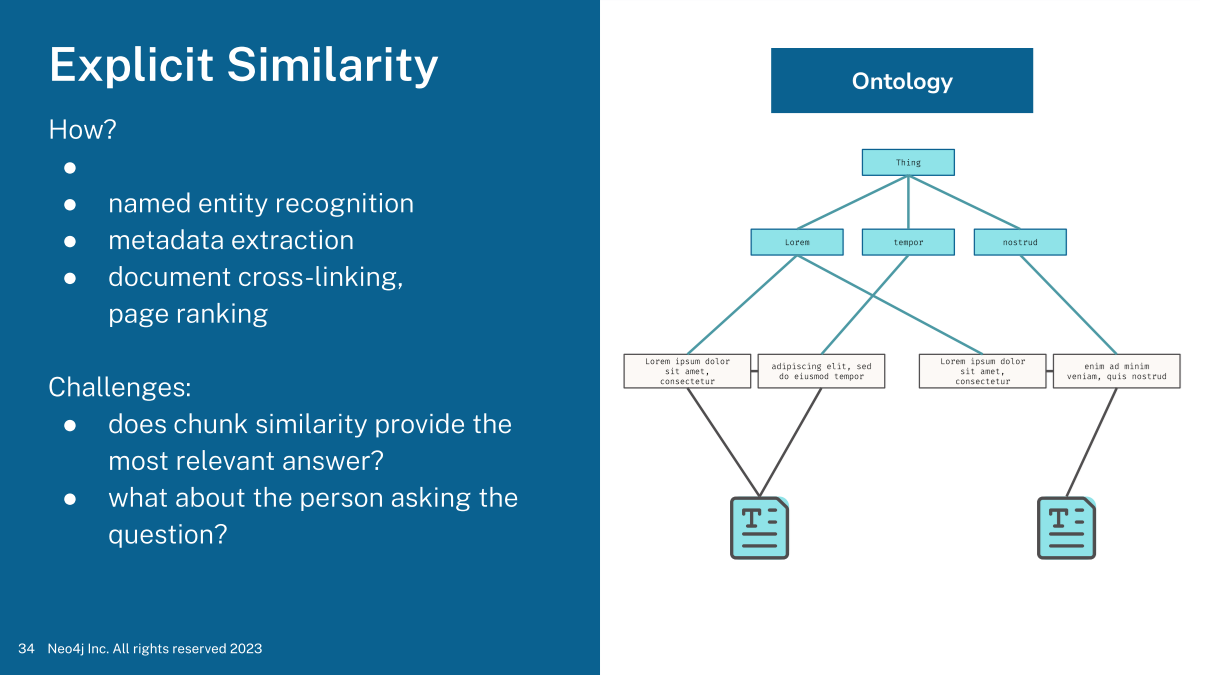
\includegraphics[width=\linewidth,keepaspectratio]{graphrag5}
	\end{center}
	
\end{frame}

%%%%%%%%%%%%%%%%%%%%%%%%%%%%%%%%%%%%%%%%%%%%%%%%%%%%%%%%%%%
\begin{frame}[fragile]\frametitle{}

	\begin{center}
	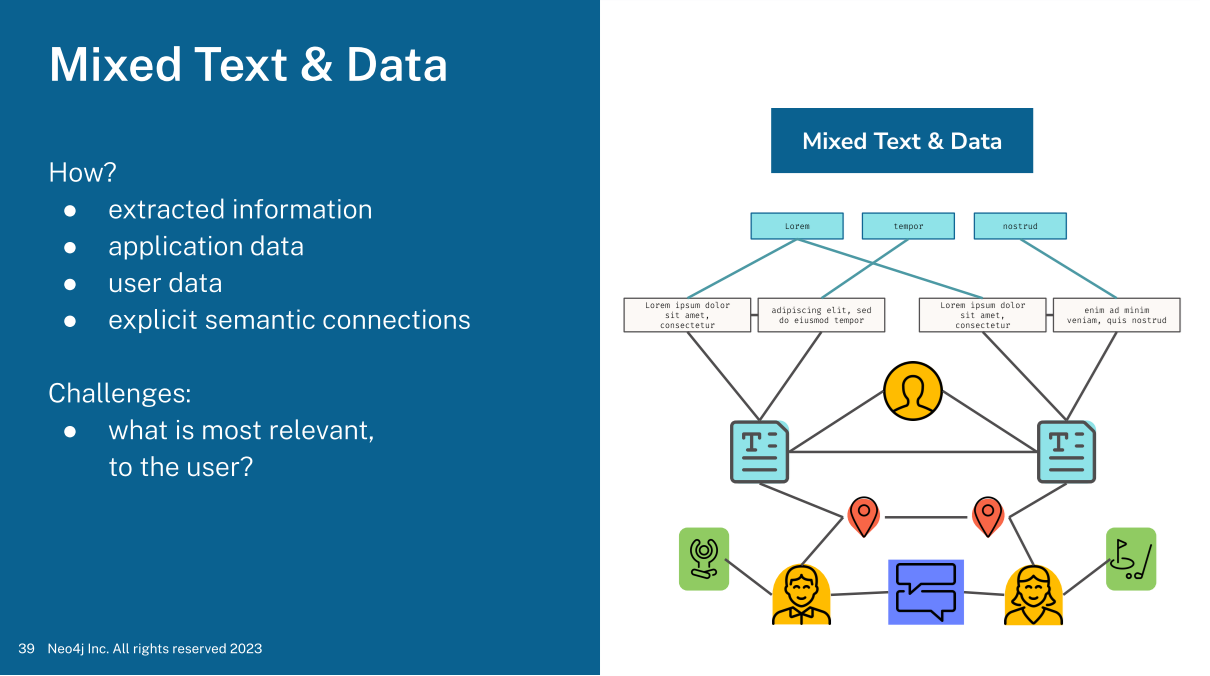
\includegraphics[width=\linewidth,keepaspectratio]{graphrag6}
	\end{center}
	
\end{frame}

%%%%%%%%%%%%%%%%%%%%%%%%%%%%%%%%%%%%%%%%%%%%%%%%%%%%%%%%%%%%%%%%%%%%%%%%%%%%%%%%%%
\begin{frame}[fragile]\frametitle{}
\begin{center}
{\Large Knowledge Graphs}
\end{center}
\end{frame}

%%%%%%%%%%%%%%%%%%%%%%%%%%%%%%%%%%%%%%%%%%%%%%%%%%%%%%%%%%%
\begin{frame}[fragile]\frametitle{}
    \begin{block}{Definition}
A Knowledge Graph is a structured way of representing 
information, typically using nodes and edges to depict 
relationships between entities (e.g., people, places, 
things, concepts). 
These entities and their interconnections form a 
graph-like structure, which can be used to model 
complex sets of data and the relationships within that 
data.
    \end{block}
	
	{\tiny (Ref: The GenAI Stack - Andreas Kollegger - Neo4j)}
	
\end{frame}


%%%%%%%%%%%%%%%%%%%%%%%%%%%%%%%%%%%%%%%%%%%%%%%%%%%%%%%%%%%
\begin{frame}[fragile]\frametitle{}

	\begin{center}
	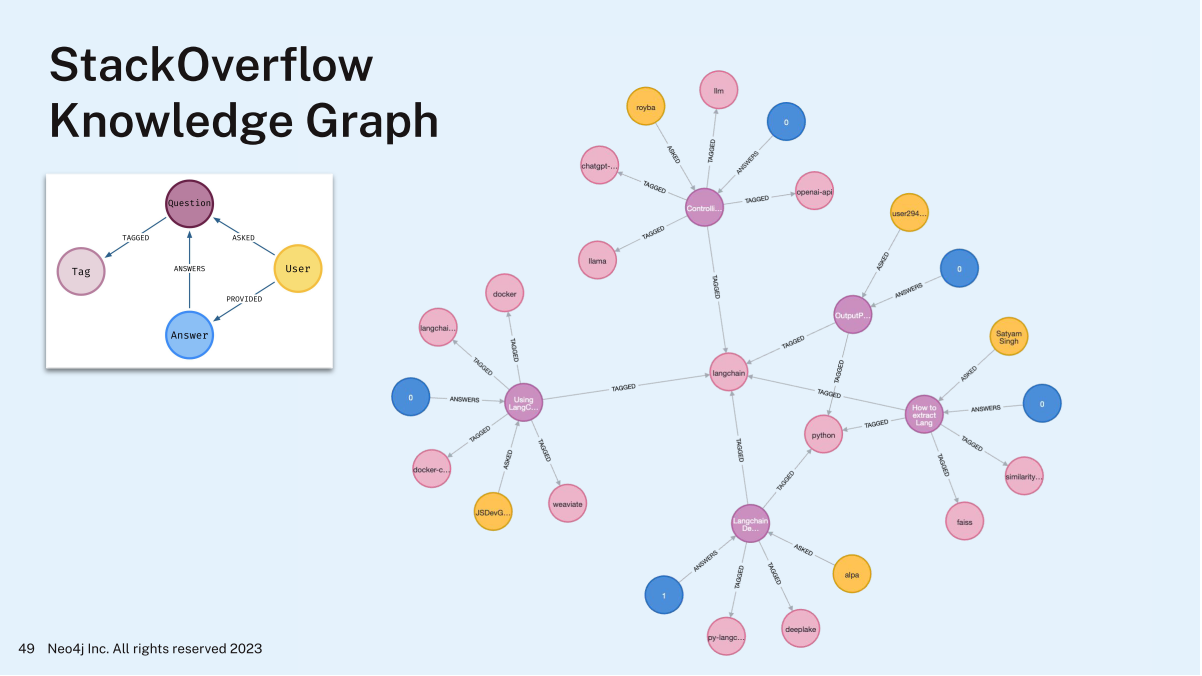
\includegraphics[width=\linewidth,keepaspectratio]{graphrag7}
	\end{center}
	
\end{frame}

%%%%%%%%%%%%%%%%%%%%%%%%%%%%%%%%%%%%%%%%%%%%%%%%%%%%%%%%%%%
\begin{frame}[fragile]\frametitle{}

	\begin{center}
	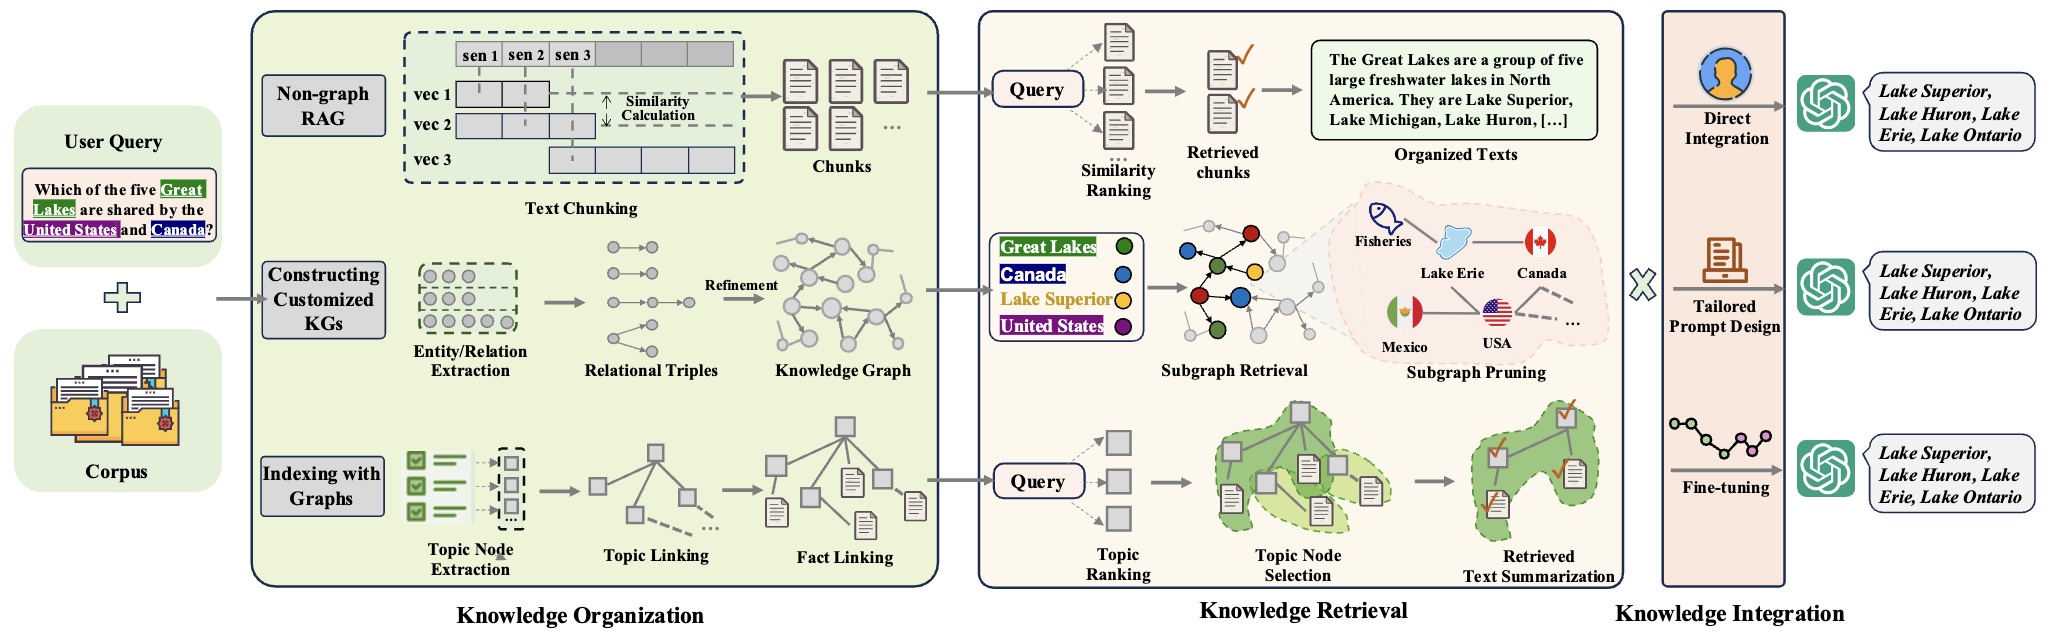
\includegraphics[width=\linewidth,keepaspectratio]{graphrag11}
	\end{center}
	
\end{frame}


%%%%%%%%%%%%%%%%%%%%%%%%%%%%%%%%%%%%%%%%%%%%%%%%%%%%%%%%%%%
\begin{frame}[fragile]\frametitle{Overview}

Overview of traditional RAG and two typical GraphRAG workflows.

    \begin{itemize}
        \item Non-graph RAG organizes the corpus into chunks, ranks them by similarity, and retrieves the most relevant text for generating responses.
        \item Knowledge-based GraphRAG extracts detailed knowledge graphs from the corpus using entity recognition and relation extraction, offering fine-grained, domain-specific information.
        \item Index-based GraphRAG summarizes the corpus into high-level topic nodes, which are linked to form an index graph, while the fact linking maps topics to text.
    \end{itemize}
	
	{\tiny (Ref: Awesome-GraphRAG (GraphRAG Survey))}
	
\end{frame}

%%%%%%%%%%%%%%%%%%%%%%%%%%%%%%%%%%%%%%%%%%%%%%%%%%%%%%%%%%%
\begin{frame}[fragile]\frametitle{Microsoft GraphRAG Workflow}

	
	\begin{center}
	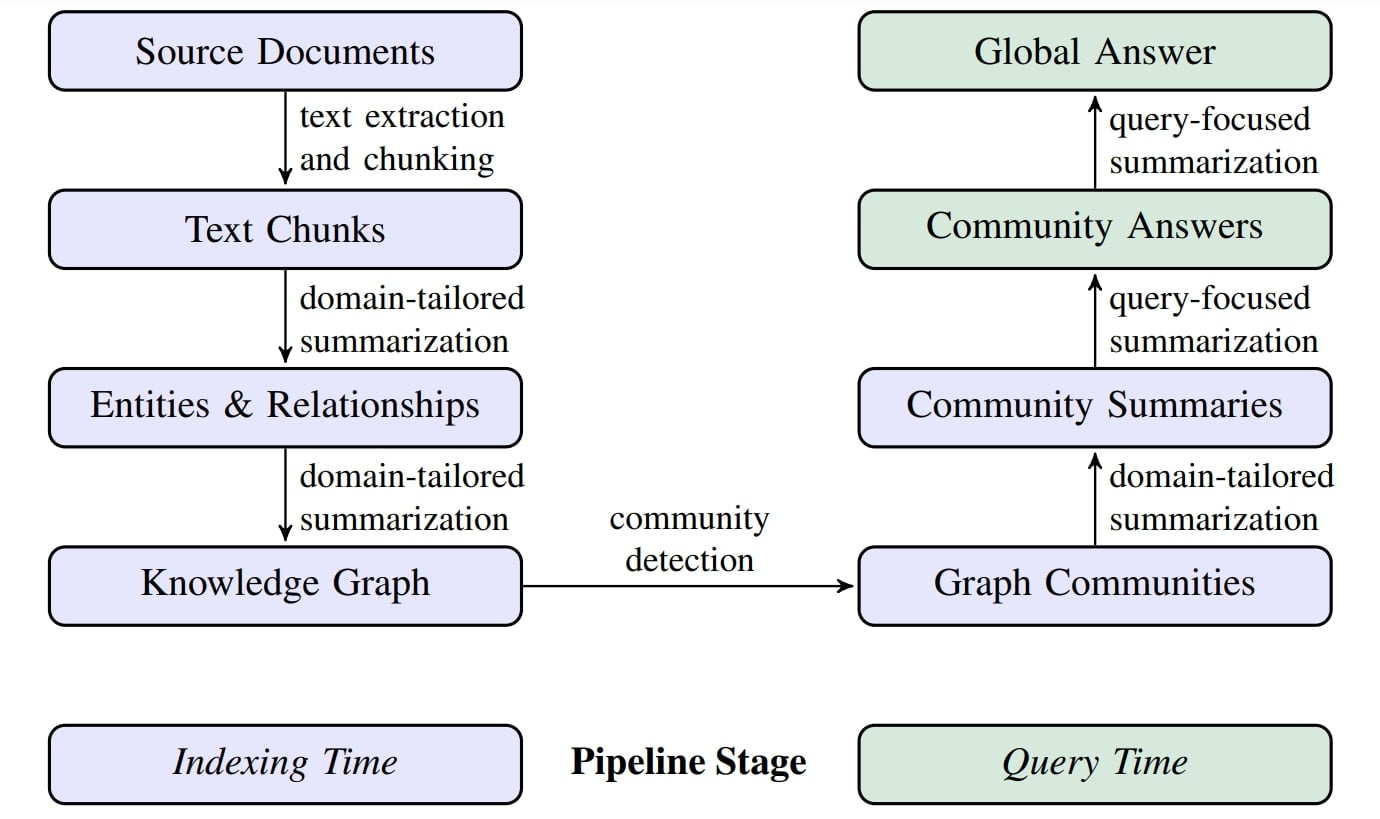
\includegraphics[width=\linewidth,keepaspectratio]{graphrag18}
	
	{\tiny (Ref: GraphRAG: The Practical Guide for Cost-Effective Document Analysis with Knowledge Graphs -Jaykumaran)}
	\end{center}	
\end{frame}

%%%%%%%%%%%%%%%%%%%%%%%%%%%%%%%%%%%%%%%%%%%%%%%%%%%%%%%%%%%
\begin{frame}[fragile]\frametitle{Indexing Phase Overview}
    \begin{itemize}
        \item Two-stage process: Generate Knowledge Graph (KG) and Community Clustering.
        \item Extract entities and relationships, construct KG.
        \item Partition KG into semantically related clusters.
        \item Generate community summaries for optimized retrieval.
    \end{itemize}
\end{frame}

%%%%%%%%%%%%%%%%%%%%%%%%%%%%%%%%%%%%%%%%%%%%%%%%%%%%%%%%%%%
\begin{frame}[fragile]\frametitle{Step 1: Segment Documents into Chunks}
    \begin{itemize}
        \item Large text split into smaller chunks for LLM processing.
        \item Small chunks retain details but increase API cost.
        \item Larger chunks reduce cost but may omit key data.
        \item Self-reflection in prompts improves extraction accuracy.
    \end{itemize}
\end{frame}

%%%%%%%%%%%%%%%%%%%%%%%%%%%%%%%%%%%%%%%%%%%%%%%%%%%%%%%%%%%
\begin{frame}[fragile]\frametitle{Step 2: Extract Entities and Relationships}
    \begin{itemize}
        \item LLM extracts entities, relationships, and descriptions.
        \item Entities assigned unique IDs for traceability.
        \item Pronouns and ambiguities resolved.
    \end{itemize}

    \begin{lstlisting}
    {
      "nodes": [
        {"id": "n0", "entity_type": "PATIENT", "name": "71-YEAR-OLD GENTLEMEN"},
        {"id": "n1", "entity_type": "DIAGNOSIS", "name": "PERIPHERAL VASCULAR DISEASE"}
      ],
      "edges": [
        {"id": "e0", "source": "n0", "target": "n1", "description": "Patient has history of this condition"}
      ]
    }
    \end{lstlisting}
\end{frame}

%%%%%%%%%%%%%%%%%%%%%%%%%%%%%%%%%%%%%%%%%%%%%%%%%%%%%%%%%%%
\begin{frame}[fragile]\frametitle{Step 2: Extract Entities and Relationships}

    \begin{lstlisting}
**-Goal-**
Given a text document that is potentially relevant to this activity and a list of entity types, identify all entities of those types from the text and all relationships among the identified entities.
 
-Steps-
1. Identify all entities. For each identified entity, extract the following information:
- entity_name: Name of the entity, capitalized
- entity_type: One of the following types: [{entity_types}]
- entity_description: Comprehensive description of the entity's 

2. From the entities identified in step 1, identify all pairs of (source_entity, target_entity) that are *clearly related to each other.
 
For each pair of related entities, extract the following information:
- source_entity: name of the source entity, as identified in step 1
- target_entity: name of the target entity, as identified in step 1
- relationship_description: explanation as to why you think the source entity and the target entity are related to each other
- relationship_strength: a numeric score indicating strength of the relationship between the source entity and target entity
    \end{lstlisting}
\end{frame}


%%%%%%%%%%%%%%%%%%%%%%%%%%%%%%%%%%%%%%%%%%%%%%%%%%%%%%%%%%%
\begin{frame}[fragile]\frametitle{Step 2: Extract Entities and Relationships}

    \begin{lstlisting}
# Entities: 
{
  "nodes": [
    {
      "id": "n0",
      "entity_type": "PATIENT",
      "description": "A male patient aged 71 with several medical conditions",
      "source_id": "n0",
      "name": "71-YEAR-OLD GENTLEMEN"
    },
    {
      "id": "n1",
      "entity_type": "DIAGNOSIS",
      "description": "Condition treated with right leg angioplasty\nPeripheral vascular disease (PVD) is a circulatory condition characterized by narrowed or blocked arteries outside of the heart and brain, leading to reduced blood flow, particularly to limbs. Patients with PVD may have undergone procedures like angioplasty in affected areas to improve circulation. Treatment generally involves medications such as Plavix and aspirin, as well as surgical interventions based on individual assessments.",
      "source_id": "n1",
      "name": "PERIPHERAL VASCULAR DISEASE"
    },
    \end{lstlisting}
\end{frame}


%%%%%%%%%%%%%%%%%%%%%%%%%%%%%%%%%%%%%%%%%%%%%%%%%%%%%%%%%%%
\begin{frame}[fragile]\frametitle{Step 2: Extract Entities and Relationships}

    \begin{lstlisting}
# Relations
 "edges": [
    {
      "id": e0,
      "source": "n0",
      "target": "n1",
      "description": "The patient has a medical history of this condition",
    },
    {
      "id": e1,
      "source": "n0",
      "target": "n2",
      "description": "Chronic Obstructive Pulmonary Disease is part of his health profile",
    },
    \end{lstlisting}
\end{frame}


%%%%%%%%%%%%%%%%%%%%%%%%%%%%%%%%%%%%%%%%%%%%%%%%%%%%%%%%%%%
\begin{frame}[fragile]\frametitle{Step 3: Construct Knowledge Graph}
    \begin{itemize}
        \item Entities and relationships aggregated into a unified KG.
        \item Duplicates merged for efficiency.
    \end{itemize}
\end{frame}

%%%%%%%%%%%%%%%%%%%%%%%%%%%%%%%%%%%%%%%%%%%%%%%%%%%%%%%%%%%
\begin{frame}[fragile]\frametitle{Step 4: Graph Partitioning into Communities}
    \begin{itemize}
        \item Leiden algorithm partitions KG into clusters.
        \item Hierarchical approach ensures fine granularity.
        \item Nodes belong to only one community.
        \item Dynamic community selection at multiple levels.
    \end{itemize}
	
	\begin{center}
	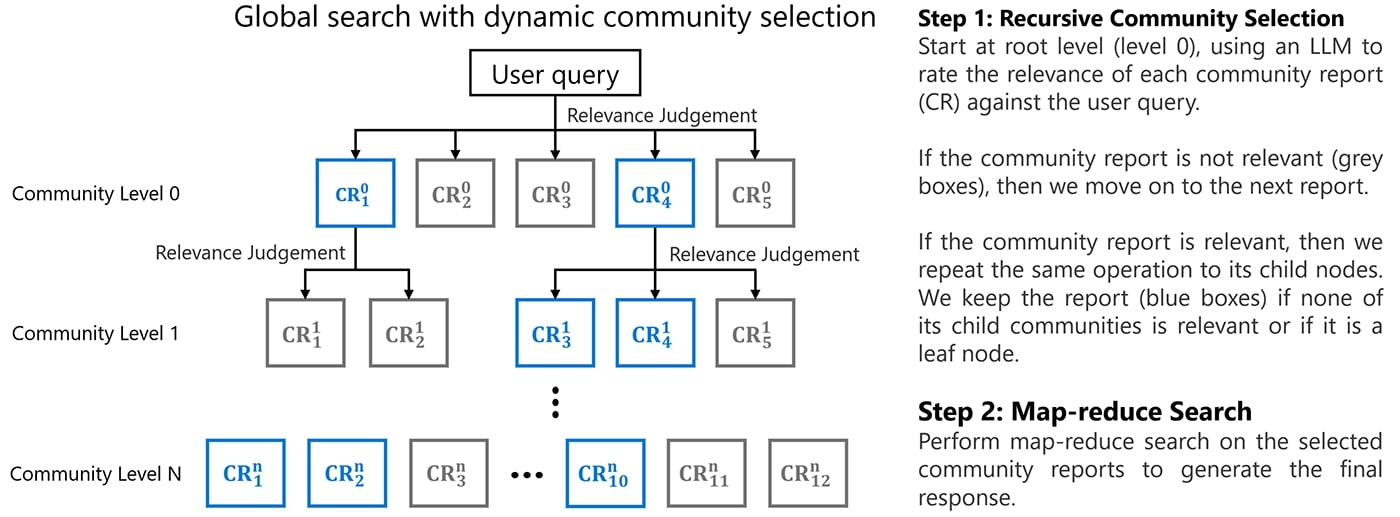
\includegraphics[width=\linewidth,keepaspectratio]{graphrag19}
	
	{\tiny (Ref: GraphRAG: The Practical Guide for Cost-Effective Document Analysis with Knowledge Graphs -Jaykumaran)}
	\end{center}	
\end{frame}

%%%%%%%%%%%%%%%%%%%%%%%%%%%%%%%%%%%%%%%%%%%%%%%%%%%%%%%%%%%
\begin{frame}[fragile]\frametitle{Step 5: Community Summarization}

    \begin{lstlisting}[language=markdown]
# **Goal**
Write a comprehensive report of a community, given a list of entities that belong to the community as well as their relationships and optional associated claims. The report will be used to inform decision-makers about information associated with the community and their potential impact. The content of this report includes an overview of the community's key entities, their legal compliance, technical capabilities, reputation, and noteworthy claims.

    \end{lstlisting}	
\end{frame}

%%%%%%%%%%%%%%%%%%%%%%%%%%%%%%%%%%%%%%%%%%%%%%%%%%%%%%%%%%%
\begin{frame}[fragile]\frametitle{Step 5: Community Summarization}

    \begin{lstlisting}[language=markdown]
# Report Structure
The report should include the following sections:
 
- TITLE: community's name that represents its key entities 
- SUMMARY: An executive summary of the community's overall structure,
- IMPACT SEVERITY RATING: a float score between 0-10 that represents the severity of IMPACT posed by entities within the community. 
- RATING EXPLANATION: Give a single sentence explanation of the IMPACT severity rating.
- DETAILED FINDINGS: A list of 5-10 key insights about the community.
    \end{lstlisting}	
\end{frame}

%%%%%%%%%%%%%%%%%%%%%%%%%%%%%%%%%%%%%%%%%%%%%%%%%%%%%%%%%%%
\begin{frame}[fragile]\frametitle{Querying Phase Overview}
    \begin{itemize}
        \item Identifies key entities and relationships in queries.
        \item Retrieves relevant community summaries instead of entire KG.
    \end{itemize}
\end{frame}

%%%%%%%%%%%%%%%%%%%%%%%%%%%%%%%%%%%%%%%%%%%%%%%%%%%%%%%%%%%
\begin{frame}[fragile]\frametitle{Query Focused Summarization (QFS)}
    \begin{itemize}
        \item Identifies patterns and correlations from queries.
        \item Matches against community summaries.
        \item Optimized retrieval ensures efficient responses.
    \end{itemize}
\end{frame}

%%%%%%%%%%%%%%%%%%%%%%%%%%%%%%%%%%%%%%%%%%%%%%%%%%%%%%%%%%%
\begin{frame}[fragile]\frametitle{Map Reduce Approach}
    \begin{itemize}
        \item \textbf{Map Phase}: Generates multiple partial responses with importance scores.
        \item \textbf{Reduce Phase}: Sorts and merges top-scoring responses into a global answer.
        \item Efficiently filters search space while maintaining accuracy.
    \end{itemize}
	
	\begin{center}
	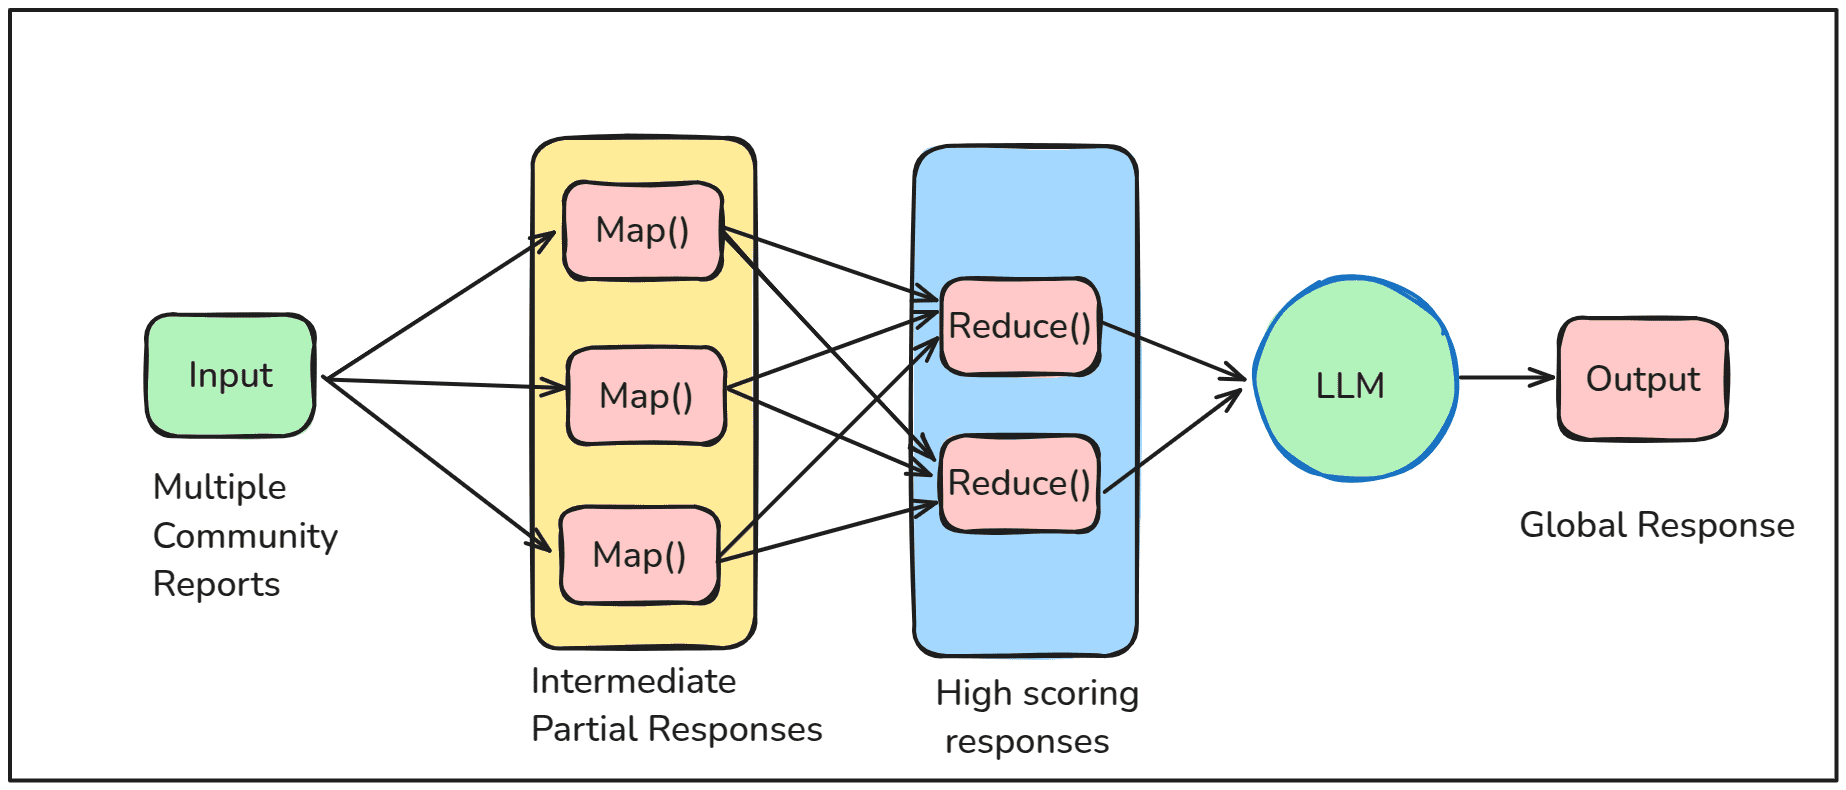
\includegraphics[width=\linewidth,keepaspectratio]{graphrag20}
	
	{\tiny (Ref: GraphRAG: The Practical Guide for Cost-Effective Document Analysis with Knowledge Graphs -Jaykumaran)}
	\end{center}		
\end{frame}



%%%%%%%%%%%%%%%%%%%%%%%%%%%%%%%%%%%%%%%%%%%%%%%%%%%%%%%%%%%
\begin{frame}[fragile]\frametitle{Benchmarks and Evaluation Metrics}
    \begin{itemize}
        \item Traditional RAGAS metrics are inadequate for sensemaking queries.
        \item LLM judges responses based on:
        \begin{itemize}
            \item \textbf{Comprehensiveness}: Covers all aspects of the query.
            \item \textbf{Diversity}: Provides varied perspectives and insights.
            \item \textbf{Empowerment}: Aids decision-making without false assumptions.
            \item \textbf{Directness}: Clear, concise, and to the point.
        \end{itemize}
        \item GraphRAG excels in comprehensiveness and diversity.
        \item Naive RAG is better at generating direct answers.
    \end{itemize}
\end{frame}

%%%%%%%%%%%%%%%%%%%%%%%%%%%%%%%%%%%%%%%%%%%%%%%%%%%%%%%%%%%
\begin{frame}[fragile]\frametitle{Shortcomings of Microsoft GraphRAG}
    \begin{itemize}
        \item Multiple LLM API calls make it slow, inefficient, and costly.
        \item No de-duplication step, resulting in a noisy graph index.
        \item Upserting new data requires reconstructing the entire KG, making it impractical for production.
    \end{itemize}
\end{frame}

%%%%%%%%%%%%%%%%%%%%%%%%%%%%%%%%%%%%%%%%%%%%%%%%%%%%%%%%%%%
\begin{frame}[fragile]\frametitle{GraphRAG Alternatives and Improvements}
    \begin{itemize}
        \item Graph-based RAG is not new; earlier versions by NebulaGraph, Langchain, LlamaIndex, Neo4j.
        \item Microsoft's approach became widely accepted but has limitations.
        \item Led to new variants focusing on efficiency and accuracy.
    \end{itemize}
\end{frame}

%%%%%%%%%%%%%%%%%%%%%%%%%%%%%%%%%%%%%%%%%%%%%%%%%%%%%%%%%%%
\begin{frame}[fragile]\frametitle{GraphRAG Variants}
    \begin{itemize}
        \item \textbf{Nano-GraphRAG}: Introduced lighter, faster versions.
        \item \textbf{Top-k Selection}: Unlike map-reduce, it selects only top-k communities for efficiency.
        \item Derived versions: LightRAG, MedGraphRAG, FastGraphRAG.
        \item MedGraphRAG is challenging to adapt to OpenAI endpoints.
    \end{itemize}
\end{frame}

%%%%%%%%%%%%%%%%%%%%%%%%%%%%%%%%%%%%%%%%%%%%%%%%%%%%%%%%%%%
\begin{frame}[fragile]\frametitle{FastGraphRAG Performance}
    \begin{itemize}
        \item 27x faster and 40\% more accurate retrieval.
        \item Benchmarks (2wikimultihopQA, 101 queries):
    \end{itemize}

	
    \begin{tabular}{lccc}
        \hline
        Method & Accuracy (All) & Accuracy (Multihop) & Insertion Time (min) \\
        \hline
        VectorDB & 0.42 & 0.23 & $\sim$0.3 \\
        LightRAG & 0.45 & 0.28 & $\sim$25 \\
        GraphRAG & 0.73 & 0.64 & $\sim$40 \\
        FastGraphRAG & 0.93 & 0.90 & $\sim$1.5 \\
        \hline
    \end{tabular}	
	
	{\tiny (Ref: GraphRAG: The Practical Guide for Cost-Effective Document Analysis with Knowledge Graphs -Jaykumaran)}	
\end{frame}

%%%%%%%%%%%%%%%%%%%%%%%%%%%%%%%%%%%%%%%%%%%%%%%%%%%%%%%%%%%
\begin{frame}[fragile]\frametitle{Graph Construction Economy Principle}
    \begin{itemize}
        \item Complex graphs require significant computational resources.
        \item Trade-off: Performance gains must justify resource investment.
        \item Aim: Maximize performance-to-resource ratio.
    \end{itemize}
\end{frame}

%%%%%%%%%%%%%%%%%%%%%%%%%%%%%%%%%%%%%%%%%%%%%%%%%%%%%%%%%%%
\begin{frame}[fragile]\frametitle{FastGraphRAG at Inference Time}
    \begin{itemize}
        \item Uses a PageRank-like algorithm (similar to Google).
        \item Determines importance of elements in the KG.
        \item Retrieves only the most relevant entities and relationships.
        \item Produces high-quality, precise responses.
    \end{itemize}
\end{frame}

%%%%%%%%%%%%%%%%%%%%%%%%%%%%%%%%%%%%%%%%%%%%%%%%%%%%%%%%%%%
\begin{frame}[fragile]\frametitle{Evaluating FastGraphRAG for Your Use Case}
    \begin{itemize}
        \item Consider cost-to-performance ratio for your specific dataset.
        \item Assess viability based on document complexity and enterprise needs.
        \item FastGraphRAG offers a scalable approach with efficiency gains.
    \end{itemize}
\end{frame}




%%%%%%%%%%%%%%%%%%%%%%%%%%%%%%%%%%%%%%%%%%%%%%%%%%%%%%%%%%%
\begin{frame}[fragile]\frametitle{Conclusion}
    \begin{itemize}
        \item GraphRAG scales from local to global knowledge representation.
        \item Community-based summaries improve response quality.
        \item Enables optimized retrieval with hierarchical partitioning.
    \end{itemize}
\end{frame}




